\documentclass[a4paper,10pt]{report}
\usepackage[francais]{babel}
\usepackage{ucs}
\usepackage[utf8x]{inputenc}
\usepackage[T1]{fontenc}
\usepackage[pdftex]{graphicx}
\usepackage{xcolor}
\usepackage{textcomp}
\usepackage[top=2cm, bottom=2cm, left=1.5cm, right=1.5cm]{geometry}
\usepackage{amsmath} 
\usepackage{amssymb}
\usepackage{mathrsfs}
\usepackage{graphicx}
\usepackage{pgfgantt}

\usepackage{listings}
\definecolor{colKeys}{rgb}{0,0,1}
\definecolor{colIdentifier}{rgb}{0,0,0}
\definecolor{-}{rgb}{0,0.5,1}
\definecolor{colString}{rgb}{0.6,0.1,0.1}
\definecolor{colBack}{rgb}{0.9,0.9,0.9}
\definecolor{colComments}{rgb}{0.5,0.5,0.5}
\definecolor{mygreen}{RGB}{28,172,0} % color values Red, Green, Blue
\definecolor{mylilas}{RGB}{170,55,241}


\lstdefinestyle{customc}
{
  belowcaptionskip=1\baselineskip,
  breaklines=true,
  frame=L,
  xleftmargin=\parindent,
  language=C,
  numbers=left,
  showstringspaces=false,
  basicstyle=\footnotesize\ttfamily,
  keywordstyle=\bfseries\color{green!40!black},
  commentstyle=\itshape\color{purple!40!black},
  identifierstyle=\color{blue},
  stringstyle=\color{orange},
  tabsize=4,
}

\lstdefinestyle{customasm}
{
  belowcaptionskip=1\baselineskip,
  frame=L,
  xleftmargin=\parindent,
  language=[x86masm]Assembler,
  basicstyle=\footnotesize\ttfamily,
  commentstyle=\itshape\color{purple!40!black},
}

\lstset{language=Matlab,%
    %basicstyle=\color{red},
    breaklines=true,%
    morekeywords={matlab2tikz},
    keywordstyle=\color{blue},%
    morekeywords=[2]{1}, keywordstyle=[2]{\color{black}},
    identifierstyle=\color{black},%
    stringstyle=\color{mylilas},
    commentstyle=\color{mygreen},%
    showstringspaces=false,%without this there will be a symbol in the places where there is a space
    numbers=left,%
    numberstyle={\tiny \color{black}},% size of the numbers
    numbersep=9pt, % this defines how far the numbers are from the text
    emph=[1]{for,end,break},emphstyle=[1]\color{red}, %some words to emphasise
    %emph=[2]{word1,word2}, emphstyle=[2]{style},    
}

\lstset{escapechar=@,style=customc}

% Title Page
\title{Rapport MT44\\\huge{TP2}}
\author{Nicolas Fleurot\\Tony Duong}

\begin{document}
\maketitle

\tableofcontents

\chapter*{Introduction}
\addcontentsline{toc}{chapter}{Introduction}

Les courbes de Bézier ont été inventées en 1962 par Pierre Bézier, ingénieur chez Renault. Les courbes de Bézier sont des courbes polynomiales paramétriques qui ont été utilisées à l’origine pour concevoir des pièces d’automobile à l’aide d’ordinateurs. Le dessin vectoriel, la CAO et toutes les activités de design industriel à partir de “dessin” sur ordinateur s’appuient sur la construction géométrique des courbes de Béziers. Aujourd’hui, elles ont de nombreuses applications dans la synthèse d’images et le rendu de polices de caractères. \\

Après les courbes de Bézier, nous nous intéressons aux courbes splines. Les B-splines sont une généralisation des courbes de Bézier et offrent beaucoup plus de souplesse en terme de manipulation et de réalisation. Elles permettent également de réaliser des courbes que les Bézier ne peuvent pas. \\

Dans une première partie, nous nous intéresserons aux courbes de Bézier et à leur construction. Pour cela, nous étudierons l’algorithme de Casteljau et l’implémenterons afin de pouvoir créer des courbes à partir de points de contrôle.\\

Dans une seconde partie, après les courbes de Bézier, nous passerons aux courbes splines et étudierons leur construction. En s’inspirant de l’algorithme de de Boor-Cox, nous créerons une fonction permettant de construire et d’afficher les B-splines de degré variable pour un vecteur noeud donné.\\

Enfin, on illustrera l’utilisation des courbes de Bézier en dessinant la lettre alpha en utilisant une Bézier de degré trois (donc avec quatre points de contrôle $P0$, $P1$, $P2$, $P3$). On dilatera et rotatera cette lettre en modifiant les positions des points de contrôle.

\chapter*{Partie 1 : Algorithme de de Casteljau}
\addcontentsline{toc}{chapter}{Partie 1 : Algorithme de de Casteljau}

\section*{Question 1a et 1b}
\addcontentsline{toc}{section}{Question 1a}

\subsection*{Rappel}
\addcontentsline{toc}{subsection}{Rappel}

On rappelle qu'il s'agit de l'algorithme classiquement utilisé pour la création des courbes de Bézier.

Il a été fourni et étudié en cours. Nous en rappelons la structure ci-dessous ; 
on définit la fonction $casteljau(P_{0} , ..., P_{n}, t \rightarrow P_{n}^{n}(t))$ comme suit :

\textbf{entrée :}

\begin{list}{}{}
\item $n+1$ points $P_{0}$, ..., $P_{n}$ de $\varepsilon$ par leurs coordonnées dans le repère ($O, \vec{i}, \vec{j}, \vec{k}$).
\item $t$ réel élément de $[0, 1]$

\end{list}

\textbf{sortie :} Coordonnées de $P^{n}_{n}(t)$\\

\textbf{Corps d'algorithme}

Début
\begin{list}{}{}
\item Initialisation\\Pour tout $i$ : $P_{i}^{0} \leftarrow P_{i}$
\item \textbf{pour} r = 0 jusqu'à $n-1$ \textbf{faire}
\item \begin{list}{}{}
\item \textbf{pour} i = r jusqu'à $n-1$ \textbf{faire}
\item \begin{list}{}{}
\item $P^{r+1}_{i+1}(t) \leftarrow (1 - t)P^{r}_{i}(t) + tP^{r}_{i+1}(t)$
\end{list}
\item \textbf{fin pour}
\end{list}
\item \textbf{fin pour}
\item Sortie de $P^{n}_{n}(t)$
\end{list}

\textbf{Fin du corps}

\subsection*{Théorie}
\addcontentsline{toc}{subsection}{Théorie}

Pour construire une courbe de Bézier, on aura besoin d’un ensemble de points de contrôles $P_{0}, P_{1}, P_{2}, …, P_{n}$ et d’un paramètre $t$ appartenant à $[0,1]$. Grâce à ces points de contrôle d’origine, nous pourrons construire des points de contrôle “fils” qui à leur tour, permettrons de construire encore d’autres points de contrôle. 

Dans le cas général, la relation liant les $P$ de rang $r$ et les $P $de rang $r-1$ est 

\begin{equation}
    P^{r}_{i+1}(t) = (1-t)P^{r-1}_{i}(t)+tP^{r-1}_{i+1}(t), r \in [1, n], i \in [r, n]
\end{equation}

Après cette explication théorique, nous implémentons l’algorithme de Casteljau afin de générer tous ces points Pn,n et ainsi afficher la courbe générée.
    
\newpage
\subsection*{Source}
\addcontentsline{toc}{subsection}{Source}

\begin{center}
	\lstinputlisting[caption=, language=Matlab]{CastelJau.m}
\end{center}

\subsection*{Test}
\addcontentsline{toc}{subsection}{Test}

\begin{center}
%	\lstinputlisting[caption=Test evaluation1, language=Matlab]{testevaluation1.m}
\end{center}

\newpage
\section*{Question 1c}
\addcontentsline{toc}{section}{Question 1b}

\subsection*{Rappel}
\addcontentsline{toc}{subsection}{Rappel}

Proposer une visualisation des points de contrôle $P_{0} , ..., P_{n}$ et de la naissance des points $P_{n}^{n}(t)$. 

\subsection*{Théorie}
\addcontentsline{toc}{subsection}{Théorie}

\begin{figure}[h]
	\begin{center}
		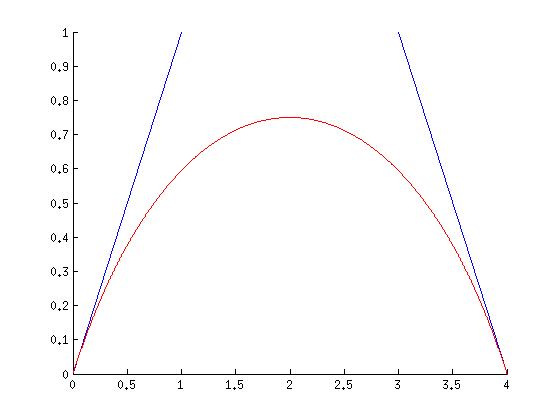
\includegraphics[scale=0.8]{visualiseCastle}
		\caption{Courbe de bézier de 4 points}
	\end{center}
\end{figure}


\subsection*{Source}
\addcontentsline{toc}{subsection}{Source}

\begin{center}
	\lstinputlisting[caption=VisualiseCastelJau.m, language=Matlab]{VisualiseCastelJau.m}
\end{center}

\subsection*{Test}
\addcontentsline{toc}{subsection}{Test}

\newpage
\section*{Question 1d}
\addcontentsline{toc}{section}{Question 1b}

\subsection*{Rappel}
\addcontentsline{toc}{subsection}{Rappel}

Que proposeriez-vous comme logiciel de démonstration, destiné à faire saisir à un étudiant qui découvre les Bézier, la manière dont se construisent les points relatifs à chaque valeur de t ?
\subsection*{Théorie}
\addcontentsline{toc}{subsection}{Théorie}

\begin{figure}[h]
	\begin{center}
		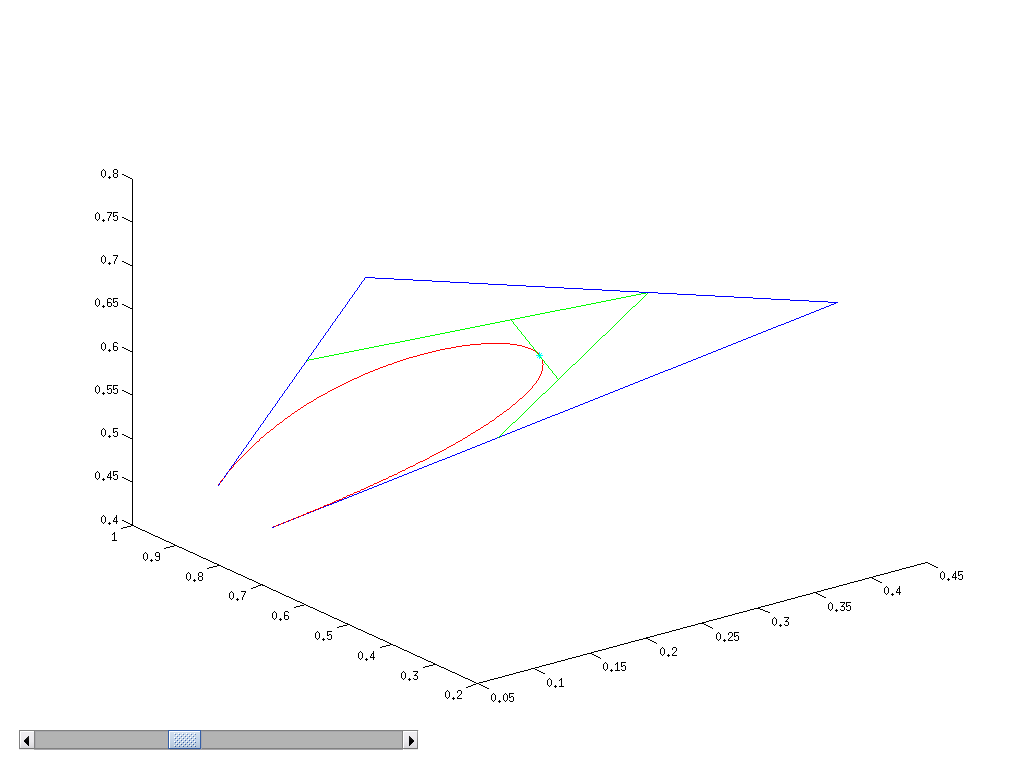
\includegraphics[scale=0.6]{guiCastle}
		\caption{Courbe de bézier de 4 points}
	\end{center}
\end{figure}


\subsection*{Source}
\addcontentsline{toc}{subsection}{Source}

\begin{center}
	\lstinputlisting[caption=, language=Matlab, mathescape]{GUICastleJauTex.m}
\end{center}

\subsection*{Test}
\addcontentsline{toc}{subsection}{Test}

\subsubsection*{Algorithme de Horner}

\textbf{entrée :}

\begin{list}{}{}
\item $n$ : entier naturel représentant le degré de $p$;
\item $a$ : vecteur de $n+1$ réels désignant les coefficients de $p$ dans la base considérée, donc $a(i) = a_{i}$ pour tout $i$ de $\lbrace 0, ..., n\rbrace$;
\item $c$ : vecteur de $n$ réels désignant les centres considérés, donc $c(i)=c_{i}$ pour tout $i$ de $\lbrace 1, ..., n\rbrace$;
\item $t$ : réel en lequel on évalue $p$;
\end{list}

\textbf{sortie}
\begin{list}{}{}
\item $val$ : réel défini par $val = p(t)$;
\item $a'$ : vecteur de $n+1$ réels, dont la signification profonde et l'utilité seront saisie dans le théorème 1.9;
\end{list}

\textbf{Début du corps}
\begin{list}{}{}
\item $a'(n) \longleftarrow a(n)$
\item \textbf{pour} i = n-1 à \textbf{faire}
\item \begin{list}{}{}
\item $a'(i) \longleftarrow a(i) + (t-c(i+1))a'(i+1)$
\end{list}
\item \textbf{fin pour}
\item $val \longleftarrow a'(0)$
\end{list}

\textbf{Fin du corps}

Nous étudierons ultérieurement la différence de performance entre ces deux schémas. 

\newpage
\subsection*{Source}
\addcontentsline{toc}{subsection}{Source}

%\lstinputlisting[caption=product, language=Matlab]{evaluation.m}

\subsection*{Test}
\addcontentsline{toc}{subsection}{Test}

\begin{center}
%	\lstinputlisting[caption=Test evaluation, language=Matlab]{testevaluation.m}
\end{center}

\section*{Question 1c}
\addcontentsline{toc}{section}{Question 1c}

\subsection*{Théorie}
\addcontentsline{toc}{subsection}{Théorie}

En utilisant les outils de Matlab $(tic, toc, etime, etc...)$ comparer les temps
d’exécution des deux fonctions d’évaluation écrites, en fonction du degré
du polynôme considéré. Visualiser les résultats obtenus.

\subsection*{Rappel}
\addcontentsline{toc}{subsection}{Rappel}

La performance est souvent très importante dans le calcul scientifique. C’est pourquoi nous comparons les temps d’exécution des deux algorithmes précédents en utilisant les fonctions tic et toc de Matlab.

\subsection*{Source / Test}
\addcontentsline{toc}{subsection}{Source / Test}

\begin{center}
%	\lstinputlisting[caption=ExecTime1, language=Matlab]{ExecTime1.m}
\end{center}

\section*{Question 1d}
\addcontentsline{toc}{section}{Question 1d}

\subsection*{Théorie}
\addcontentsline{toc}{subsection}{Théorie}

Ecrire une version matricielle de $evaluation()$, qui à partir d’un vecteur
colonne de réels $T$ produit le vecteur colonne des images $p(T)$. Cette nouvelle
version sera conservée sous le même nom et considérée comme algorithme
d’évaluation par défaut.

\subsection*{Source}
\addcontentsline{toc}{subsection}{Source}

%\lstinputlisting[caption=product, language=Matlab]{evaluation2.m}

\subsection*{Test}
\addcontentsline{toc}{subsection}{Test}

\begin{center}
%	\lstinputlisting[caption=Test evaluation2, language=Matlab]{testevaluation2.m}
\end{center}

\chapter*{Partie 2 : Table des différences divisées et polynômes d’interpolation}
\addcontentsline{toc}{chapter}{Partie 2 : Table des différences divisées et polynômes d’interpolation}

On utilisera évidemment les algorithmes fournis en cours. On considère une
fonction $f$, connue sur un support $\lbrace x_{0},...,x_{n}\rbrace$, par la donnée pour tout $i$ de $\lbrace 0,...,n \rbrace$, de $y_{i}$ = $f(x_{i})$.

\section*{Question 2a}
\addcontentsline{toc}{section}{Question 2a}

\subsection*{Rappel}
\addcontentsline{toc}{subsection}{Rappel}

Ecrire une fonction $table\_diff\_div(x, y)$ qui, à partir des deux colonnes $x = (x_{0},...,x_{n})$ et $y = (f(x_{0}),...,f(x_{n}))$ de même taille, construit et affiche la table des différences divisées de $f$ sur le support considéré.

\subsection*{Théorie}
\addcontentsline{toc}{subsection}{Théorie}

Les différents coefficients ai de l’écriture de Newton se déterminent de la manière suivante : $a_{i} = f[x_{0},...,x_{n}] = \frac{f[x_{1},..,x_{k}]-f[x_{0},..,x_{k-1}]}{(x_{k}-x_{0})}$.
De plus, pour 1 point de support (support $\lbrace x_{0} \rbrace$), $f[x_{0}] = f(x_{0})$.
Pour 2 points de support (support $\lbrace x_{0},x_{1} \rbrace$), $f[x_{0},x_{1}] = \frac{f(x_{1})-f(x_{0})}{(x_{1}-x_{0})}$.
Ainsi, nous pouvons construire la table qui contiendra tous les coefficients de l’écriture de Newton à partir d’un support quelconque, appelé table des différences divisées.

\newpage
\subsection*{Source}
\addcontentsline{toc}{subsection}{Source}

\begin{center}
%	\lstinputlisting[caption=table\_diff\_div, language=Matlab]{table_diff_div.m}
\end{center}

\subsection*{Test}
\addcontentsline{toc}{subsection}{Test}

\begin{center}
%	\lstinputlisting[caption=Test table\_diff\_div, language=Matlab]{testtable_diff_div.m}
\end{center}

\section*{Question 2b}
\addcontentsline{toc}{section}{Question 2b}

\subsection*{Rappel}
\addcontentsline{toc}{subsection}{Rappel}

Ecrire une fonction $interpol(n, x, y)$ qui, à partir de l’entier naturel non
nul n, et des données x et y définies ci-dessus construit le vecteur des
composantes du polynôme d’interpolation $p_{n}$ de $f$ sur le support $\lbrace  x_{0},...,x_{n} \rbrace$,
ainsi que la chaîne de son écriture.

\subsection*{Théorie}
\addcontentsline{toc}{subsection}{Théorie}

Les coefficients de Newton sont situés sur la diagonale descendante de la table des différences divisées. 

L’écriture de Newton est de la forme :

\begin{equation}
p(x) = \sum_{\substack{i=0}}^{n} \left(a_{i}\left[\prod_{j=0}^{i-1}(x-x_{j})\right]\right)
\end{equation}

Ainsi, nous utilisons la fonction précédente générant la table des différences divisés afin de récupérer les coefficients de l’écriture de Newton. Après cela, nous affichons sa chaîne de caractères pour mettre en évidence sa constitution. 

\newpage
\subsection*{Source}
\addcontentsline{toc}{subsection}{Source}

\begin{center}
%	\lstinputlisting[caption=interpol, language=Matlab]{interpol.m}
\end{center}

\subsection*{Test}
\addcontentsline{toc}{subsection}{Test}

\begin{center}
%	\lstinputlisting[caption=Test interpol, language=Matlab]{testinterpol.m}
\end{center}

\section*{Question 2c}
\addcontentsline{toc}{section}{Question 2c}

\subsection*{Rappel}
\addcontentsline{toc}{subsection}{Rappel}

\begin{list}{}{}
\item \begin{list}{$\bullet$}{}
\item Déterminer le polynôme d’interpolation $p_{7,1}$ de la fonction exp sur
le support $X1$ des huits points régulièrement répartis sur l’intervalle [1, 1].
\item Déterminer le polynôme d’interpolation $p_{7,2}$ de la fonction $exp$ sur le
support $X2$ des huits points de Tchebyschev, définis par : $\forall j \in \lbrace 0,...,7 \rbrace$  $X2_{j} = cos(\frac{2j+1}{8} \frac{\pi}{2}).$
\end{list}
\end{list}

\subsection*{Théorie}
\addcontentsline{toc}{subsection}{Théorie}

Nous mettons ici en application les outils précédemment développés pour interpoler la fonction exponentielle sur deux supports différents et pour afficher les écritures respectives.

Les supports sont :
\begin{list}{}{}
\item \begin{list}{$\bullet$}{}
\item le support des huit points régulièrement répartis sur l’intervalle [-1,1].
\item le support des huit points de Tchebyschev définis par : $\forall j \in \lbrace 0,...,7 \rbrace$  $X2_{j} = cos(\frac{2j+1}{8} \frac{\pi}{2}).$

\end{list}
\end{list}

\newpage
\subsection*{Source / Test}
\addcontentsline{toc}{subsection}{Source / Test}

\begin{center}
%	\lstinputlisting[caption=ApplicationExp, language=Matlab]{ApplicationExp.m}
\end{center}

\begin{center}
%	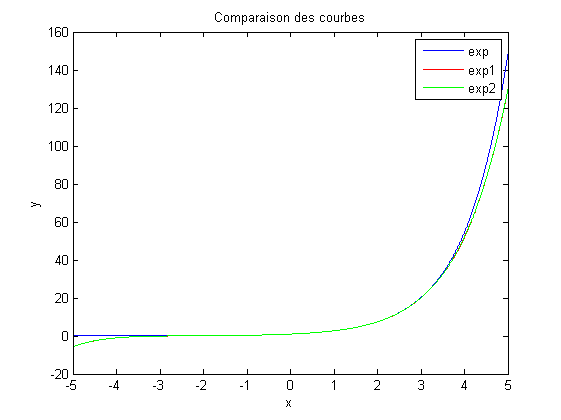
\includegraphics[scale=0.8]{comparaison.png}
\end{center}
Sur l'intervalle [-1,1], la différence est quasi-nulle.
Nous remarquons que plus on s'éloigne du domaine d'étude (ici, intervalle [-1;1]), plus la différence entre la courbe de la fonction exponentielle et celles des fonctions interpôlantes augmente. Ceci est cohérent. L'erreur entre les deux courbes et la fonction exponentielle sera étudiée plus en détail dans la partie suivante.

\chapter*{Partie 3 : Visualisation de l’erreur d’interpolation}
\addcontentsline{toc}{chapter}{Partie 3 : Visualisation de l’erreur d’interpolation}

\subsection*{Rappel}
Utiliser la question précédente et les outils antérieurement développés, pour
visualiser sur une même représentation graphique, la valeur absolue de l’erreur
d’interpolation commise lors de l’approximation de la fonction exponentielle
par $p_{7,1}$ et $p_{7,2}$.


\subsection*{Théorie}
Nous utilisons ici les outils antérieurement développés pour calculer l'erreur entre la fonction exponentielle connu et son approximation par $p_{7,1}$ et $p_{7,2}$.
Nous utiliserons la formule
\begin{equation}
	e_{n}(t) = f(t) - p_{n}(t)
\end{equation}

avec

\begin{list}{}{}
\item
\begin{itemize}
	\item[$e_{n}(t)$]: Erreur de l'approximation.
	\item[$f(t)$]: Fonction exponentielle.
	\item[$p_{n}(t)$]: Approximation de la fonction exponentielle.
\end{itemize}
\end{list}

\subsection*{Source}
\addcontentsline{toc}{subsection}{Source}
\begin{center}
%	\lstinputlisting[caption=Erreur, language=Matlab, mathescape]{Erreur.m}
\end{center}

\subsection*{Test}
\addcontentsline{toc}{subsection}{Test}

\begin{center}
%	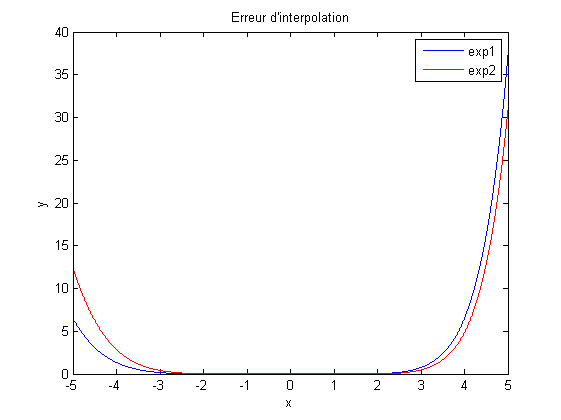
\includegraphics[scale=0.8]{erreur.png} 
\end{center}

\begin{center}
%	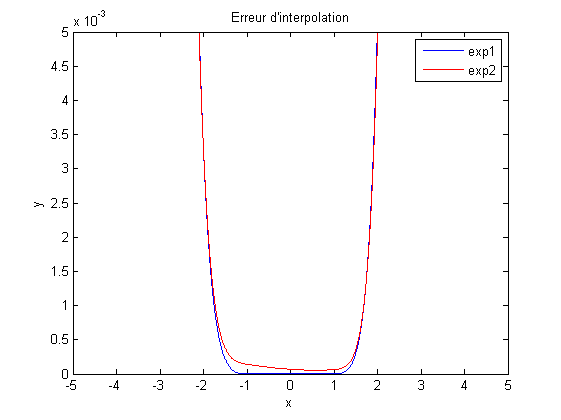
\includegraphics[scale=0.8]{zoomErreur.png} 
\end{center}

L'erreur est nulle aux points de support. Nous pouvons observer que globalement, l'erreur augmente de manière exponentielle. Néanmoins, dès que l'on s'éloigne de l'intervalle [-1,1], l'erreur avec le support de Tchebyschev devient nettement plus petite que l'erreur avec le support des points équi-distants (échelle minuscule). C'est l'avantage d'utiliser ces points si on souhaite une fonction qui approxime correctement même en dehors de l'intervalle d'étude.

\chapter*{Conclusion}
\addcontentsline{toc}{chapter}{Conclusion}

La problématique de ce chapitre a été de pouvoir trouver une fonction polynôme qui passerait par un nombre fini de points d’un certain support (obtenus par mesures par exemples). Il existe plusieurs méthodes pour arriver à ce but.
\newline
\newline
Dans ce TP, nous avons utilisé la méthode de Newton et avons produit deux algorithmes permettant d’évaluer la fonction en un point quelconque t. La fonction supposait que l’on connaissait à l’avance les coefficients de l’écriture de Newton.
\newline
\newline
Le premier algorithme produit est classique : il consiste à calculer les polynômes $(x-c)$ où $c$ est un point du support et à multiplier ceux-ci par leurs coefficients respectifs. Néanmoins, cette méthode génère des répétitions et n’est donc pas optimal en terme de temps d’éxécution.
\newline
\newline 
La seconde méthode tiré du Schéma de Horner n’a pas ce défaut. En effet, étant donné que les facteurs $(x-c)$ sont répétés dans l’écriture, il était préférable d’ajouter les facteurs déjà calculés aux les termes suivants de la somme.
\newline
\newline
La mesure du temps d’exécution confirme notre affirmation.
\newline
\newline
Par la suite, nous nous sommes intéressés par l’écriture de la fonction interpôlante en générant la table des différences divisées (qui contient les coefficients de Newton) et en écrivant cette écriture sous forme de chaîne de caractères. Nous devions ensuite interpôler la fonction exponentielle. 
\newline
\newline
Mais la question la plus importante concerne l’erreur commise en faisant cette approximation et le choix des points de support. L’erreur aux points de support est bien sûr nulle mais qu’en est-il des autres points ? 
\newline
\newline
Nous avons observé que l’erreur (pour les deux fonctions d'interpolation) grandissait au fur et à mesure qu’on s’éloignait des points de support. En ce qui concerne le choix entre les deux supports(équi-distants ou Tchebyschev), nous ne voyons pas immédiatement la différence sur l'exemple de ce TP, mais utiliser les points de Tchebyschev permet d'atténuer le phénomène de Runge qui rend "instable" la courbe d'interpolation : plus on ajoute de points sur le support, plus la courbe sera "instable" au bord. En concentrant les points de supports aux extrémités de l'intervalle, ce phénomène est affaibli et on obtient une meilleure approximation globale. 


\end{document}